% ============================================================================
% CHAPITRE 2 — LANCEMENT DE PROJET
% Structure inspirée du rapport de référence (Amal Rahmeni)
% ============================================================================

\section{Introduction}

Ce deuxième chapitre marque le lancement formel du projet Guidni selon les pratiques de la méthodologie Scrum. Il détaille l'analyse approfondie des besoins, la constitution du Product Backlog, et la définition de l'environnement de développement. Pour cela, nous avons suivi le plan suivant :

\begin{enumerate}
    \item Analyse et spécification des besoins fonctionnels et non fonctionnels
    \item Définitions théoriques des concepts clés (LLM, RAG, LinUCB)
    \item Architecture fonctionnelle et logique du système
    \item Constitution du Product Backlog
    \item Planification détaillée des Sprints
    \item Outils et environnement de développement
\end{enumerate}

La section suivante présente l'analyse détaillée des besoins du système.


% ────────────────────────────────────────────────────────────────
\section{Analyse des besoins}
% ────────────────────────────────────────────────────────────────

\subsection{Besoins fonctionnels}

L'analyse des besoins fonctionnels a été réalisée en collaboration avec l'encadrant du projet, M. Nizar Tenzekhti, et s'est concrétisée par l'identification des acteurs et la formulation de User Stories selon le format Scrum standard.

\textbf{Acteur principal : Touriste}
\begin{itemize}
    \item \textbf{US-01} : En tant que touriste, je veux envoyer des messages en langage naturel (français, anglais, arabe) pour obtenir un plan de voyage personnalisé.
    \item \textbf{US-02} : En tant que touriste, je veux recevoir un itinéraire multi-jours structuré avec activités, hébergements et restaurants.
    \item \textbf{US-03} : En tant que touriste, je veux modifier mon plan existant par des messages de suivi conversationnels.
    \item \textbf{US-04} : En tant que touriste, je veux consulter l'historique de mes conversations précédentes.
    \item \textbf{US-05} : En tant que touriste, je veux voir des recommandations personnalisées apparaître automatiquement lors de ma navigation.
\end{itemize}

\textbf{Acteur secondaire : Administrateur}
\begin{itemize}
    \item \textbf{US-06} : En tant qu'administrateur, je veux reconstruire l'index RAG via un endpoint dédié.
    \item \textbf{US-07} : En tant qu'administrateur, je veux consulter l'état de santé du système (base de données, LLM, index).
    \item \textbf{US-08} : En tant qu'administrateur, je veux sélectionner le fournisseur LLM par défaut.
\end{itemize}

\textbf{Acteur système : Processus automatisés}
\begin{itemize}
    \item \textbf{US-09} : En tant que système, je veux réindexer automatiquement les entités modifiées en base de données.
    \item \textbf{US-10} : En tant que système, je veux scorer une liste de recommandations en moins de 100~ms grâce au cache matriciel LinUCB.
    \item \textbf{US-11} : En tant que système, je veux collecter les événements comportementaux utilisateurs sans bloquer le frontend.
    \item \textbf{US-12} : En tant que système, je veux exécuter des jobs nocturnes pour mettre à jour les profils utilisateurs et rafraîchir les matrices LinUCB.
\end{itemize}

\subsection{Besoins non fonctionnels}

Les exigences non fonctionnelles suivantes ont été identifiées comme critiques pour la réussite du projet :

\begin{table}[H]
    \centering
    \caption{Exigences non fonctionnelles du système Guidni}
    \label{tab:nfr}
    \small
    \begin{tabular}{p{2cm} p{6cm} p{5cm}}
        \toprule
        \textbf{Catégorie} & \textbf{Exigence} & \textbf{Critère d'acceptation} \\
        \midrule
        Performance & Latence de réponse de l'agent < 5 secondes & Temps moyen mesuré sur 100 requêtes \\
        Performance & Latence de scoring LinUCB < 100 ms & Mesure via endpoint /health \\
        Disponibilité & Système opérationnel 99\% du temps & Monitoring continu \\
        Multilinguisme & Support FR/EN/AR natif & Tests de requêtes dans les 3 langues \\
        Scalabilité & Support de 1000 utilisateurs simultanés & Tests de charge \\
        Sécurité & Authentification JWT requise pour API & Validation des tokens \\
        Maintenabilité & Couverture de tests > 80\% & Rapport pytest-cov \\
        \bottomrule
    \end{tabular}
\end{table}


% ────────────────────────────────────────────────────────────────
\section{Définitions théoriques}
% ────────────────────────────────────────────────────────────────

\subsection{Grands Modèles de Langage (LLM)}

Les Large Language Models sont des réseaux de neurones profonds basés sur l'architecture Transformer, entraînés sur des corpus textuels massifs pour prédire le token suivant dans une séquence. Leur capacité à générer du texte cohérent et à suivre des instructions en fait des composants centraux pour les agents conversationnels.

\subsection{Retrieval-Augmented Generation (RAG)}

Le RAG est une technique hybride combinant la récupération d'informations depuis une base de connaissances externe avec la génération de texte par un LLM. Cette approche permet de fournir au modèle un contexte factuel vérifié, réduisant ainsi les hallucinations et améliorant la précision des réponses.

\subsection{Bandits Contextuels et LinUCB}

LinUCB (Linear Upper Confidence Bound) est un algorithme de bandit manchot contextuel qui apprend à sélectionner la meilleure action (recommandation) en fonction d'un vecteur de caractéristiques contextuelles. L'algorithme maintient une estimation de l'utilité attendue pour chaque action et ajoute un terme d'exploration pour découvrir de nouvelles options potentielles.

\begin{table}[H]
    \centering
    \caption{Comparaison des approches de recommandation}
    \label{tab:recommendation_comparison}
    \small
    \begin{tabular}{p{2.5cm} p{4cm} p{4cm} p{4cm}}
        \toprule
        \textbf{Approche} & \textbf{Principe} & \textbf{Points Forts} & \textbf{Limitations} \\
        \midrule
        Filtrage collaboratif & Recommande selon les similarités utilisateurs & Découvertes inattendues, pas besoin de contenu structuré & Cold start, sparsité des données \\
        Basé sur le contenu & Recommande selon similarité attributs & Pas de cold start, explications faciles & Bulles de filtres, manque de diversité \\
        LinUCB (notre choix) & Apprentissage en ligne par renforcement & Adaptation temps réel, exploration contrôlée & Complexité implémentation, tuning requis \\
        \bottomrule
    \end{tabular}
\end{table}


% ────────────────────────────────────────────────────────────────
\section{Architecture fonctionnelle}
% ────────────────────────────────────────────────────────────────

\subsection{Vue d'ensemble}

L'architecture fonctionnelle de Guidni se compose de trois couches principales :

\begin{enumerate}
    \item \textbf{Couche Présentation} : Interface Next.js avec composant de chat et widgets de recommandation
    \item \textbf{Couche Métier} : API FastAPI hébergeant l'agent LangGraph et le moteur LinUCB
    \item \textbf{Couche Données} : PostgreSQL avec extensions pgvector pour stockage relationnel et vectoriel
\end{enumerate}

\subsection{Diagramme de cas d'utilisation global}

La figure ci-dessous présente les interactions entre les acteurs et les fonctionnalités du système :

\begin{figure}[H]
    \centering
    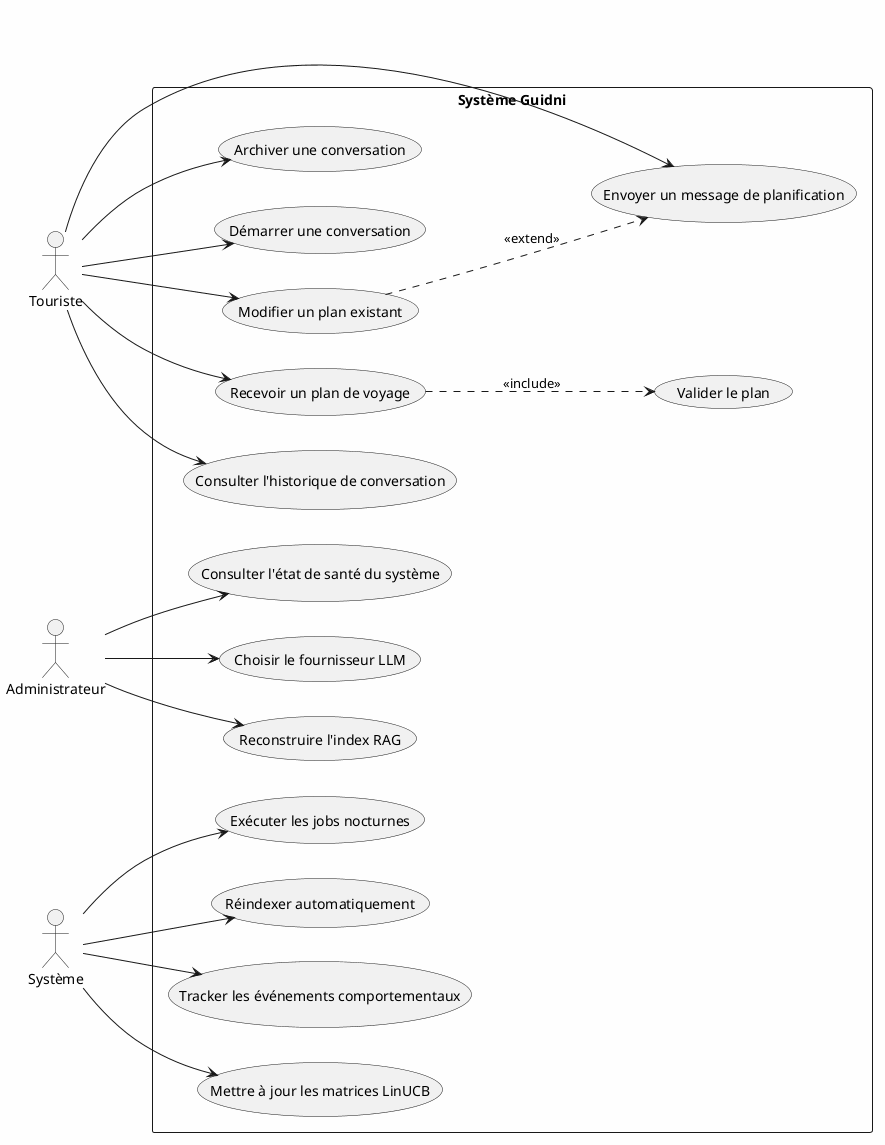
\includegraphics[width=\textwidth]{diagrams/fig_03_use_case_global.png}
    \caption{Diagramme des cas d'utilisation global}
    \label{fig:use_case_global}
\end{figure}


% ────────────────────────────────────────────────────────────────
\section{Product Backlog}
% ────────────────────────────────────────────────────────────────

Le Product Backlog initial regroupe l'ensemble des User Stories priorisées selon la méthode MoSCoW :

\begin{table}[H]
    \centering
    \caption{Product Backlog initial du projet Guidni}
    \label{tab:product_backlog}
    \small
    \begin{tabular}{p{1cm} p{7cm} p{2cm} p{3cm}}
        \toprule
        \textbf{ID} & \textbf{User Story} & \textbf{Priorité} & \textbf{Sprint cible} \\
        \midrule
        US-01 & Envoyer messages NL multilingues pour obtenir plan & Must Have & Sprint 2 \\
        US-02 & Recevoir itinéraire multi-jours structuré & Must Have & Sprint 2 \\
        US-03 & Modifier plan par messages de suivi & Should Have & Sprint 2 \\
        US-04 & Consulter historique conversations & Should Have & Sprint 2 \\
        US-05 & Voir recommandations personnalisées auto & Must Have & Sprint 4 \\
        US-06 & Reconstruire index RAG (admin) & Should Have & Sprint 3 \\
        US-07 & Consulter état santé système & Must Have & Sprint 1 \\
        US-08 & Sélectionner fournisseur LLM & Could Have & Sprint 2 \\
        US-09 & Réindexation automatique entités modifiées & Must Have & Sprint 3 \\
        US-10 & Scoring recommandations < 100 ms & Must Have & Sprint 4 \\
        US-11 & Collecte événements comportementaux & Must Have & Sprint 4 \\
        US-12 & Jobs nocturnes maintenance & Should Have & Sprint 4 \\
        \bottomrule
    \end{tabular}
\end{table}


% ────────────────────────────────────────────────────────────────
\section{Planification des Sprints}
% ────────────────────────────────────────────────────────────────

\begin{table}[H]
    \centering
    \caption{Planification détaillée des Sprints}
    \label{tab:sprint_details}
    \small
    \begin{tabular}{p{1.5cm} p{3cm} p{5cm} p{4cm}}
        \toprule
        \textbf{Release} & \textbf{Sprint} & \textbf{Objectif} & \textbf{Période} \\
        \midrule
        Release 1 & Sprint 1 & Analyse besoins + Architecture globale & Octobre 2024 \\
        Release 1 & Sprint 2 & Agent LangGraph + 18 outils & Novembre 2024 \\
        Release 2 & Sprint 3 & Pipeline RAG multilingue & Décembre 2024 \\
        Release 2 & Sprint 4 & Moteur LinUCB + Tracker & Janvier 2025 \\
        Release 3 & Sprint 5 & Tests + Évaluation + Déploiement & Février 2025 \\
        \bottomrule
    \end{tabular}
\end{table}


% ────────────────────────────────────────────────────────────────
\section{Outils et environnement}
% ────────────────────────────────────────────────────────────────

\subsection{Environnement de développement}

\begin{itemize}
    \item \textbf{Langage} : Python 3.12 pour le backend, TypeScript pour le frontend
    \item \textbf{Framework Backend} : FastAPI avec Uvicorn comme serveur ASGI
    \item \textbf{Framework Frontend} : Next.js 14 avec App Router
    \item \textbf{Base de données} : PostgreSQL 15 avec extension pgvector
    \item \textbf{Gestion de dépendances} : Poetry (Python), npm (TypeScript)
    \item \textbf{Contrôle de version} : Git avec dépôt GitHub privé
\end{itemize}

\subsection{Outils de gestion de projet}

\begin{itemize}
    \item \textbf{Suivi des tâches} : GitHub Projects avec tableaux Kanban
    \item \textbf{Documentation} : Markdown pour les spécifications techniques
    \item \textbf{Tests} : pytest pour Python, Jest pour TypeScript
    \item \textbf{CI/CD} : GitHub Actions pour l'intégration continue
\end{itemize}


% ────────────────────────────────────────────────────────────────
\section{Conclusion}
% ────────────────────────────────────────────────────────────────

Ce chapitre a formalisé le lancement du projet Guidni selon les pratiques Scrum. Nous avons identifié douze User Stories couvrant les besoins des touristes, administrateurs et processus systèmes. Les exigences non fonctionnelles ont été définies avec des critères d'acceptation mesurables. Le Product Backlog priorisé et la planification des cinq Sprints fournissent désormais une feuille de route claire pour le développement.

Le chapitre suivant détaillera l'exécution du Sprint 1, consacré à l'analyse approfondie et à la validation de l'architecture globale du système.
